% Cover 4: "Blueprint" — Technical blueprint aesthetic, midnight blue, white linework
\documentclass[tikz,border=0mm]{standalone}
\usepackage{tikz}
\usetikzlibrary{calc,patterns,decorations.pathmorphing}
\usepackage{xcolor}
\usepackage[T1]{fontenc}

\definecolor{blueprintbg}{RGB}{15,35,80}
\definecolor{blueprintline}{RGB}{100,160,240}
\definecolor{blueprintbright}{RGB}{180,215,255}
\definecolor{blueprintdim}{RGB}{50,90,160}
\definecolor{white}{RGB}{255,255,255}
\definecolor{cyanaccent}{RGB}{0,220,220}
\definecolor{yellowaccent}{RGB}{255,220,50}

\begin{document}
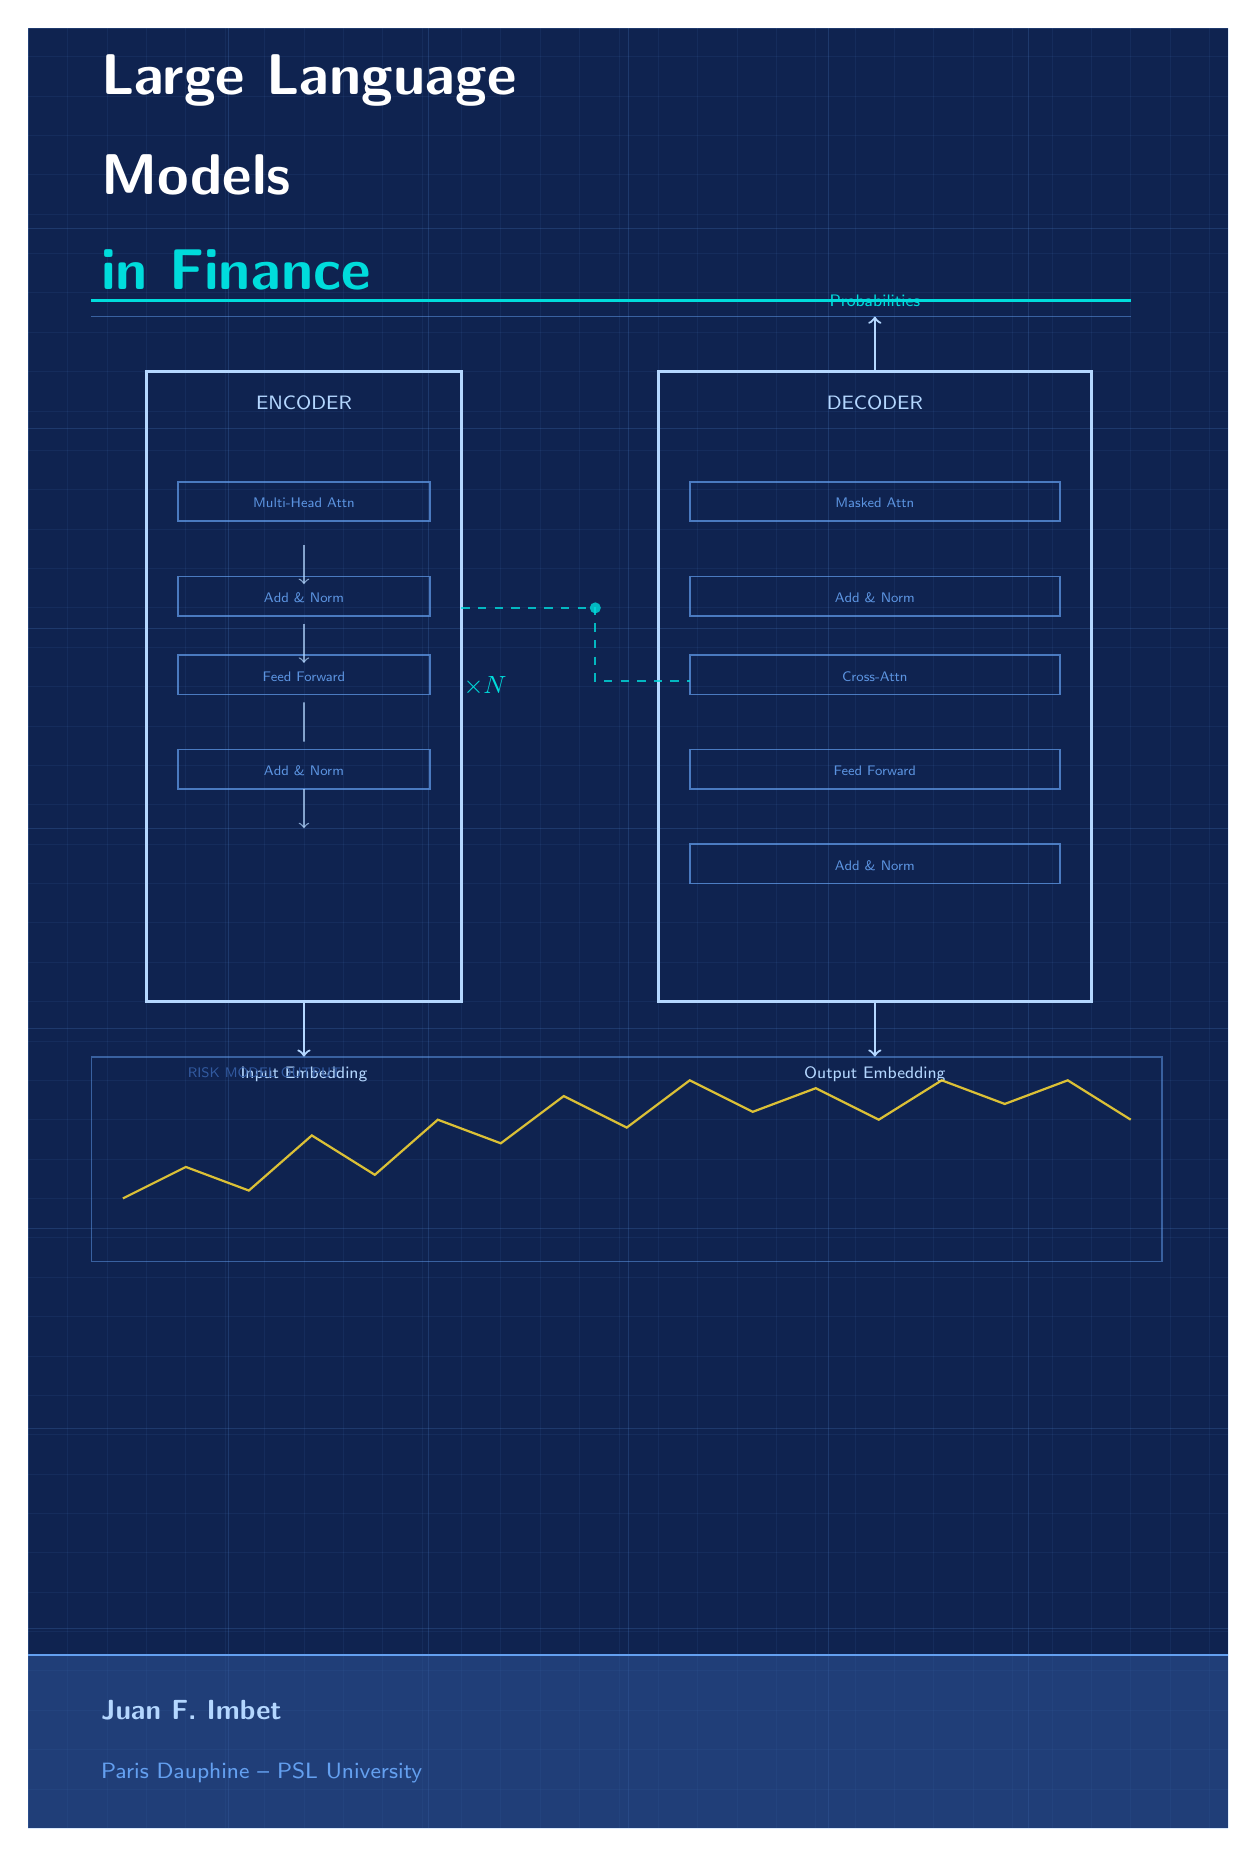
\begin{tikzpicture}
  % --- background ---
  \fill[blueprintbg] (0,0) rectangle (15.24,22.86);

  % --- blueprint grid ---
  \foreach \x in {0,0.5,...,15.24}{
    \draw[blueprintline,opacity=0.08,line width=0.3pt] (\x,0) -- (\x,22.86);
  }
  \foreach \y in {0,0.5,...,22.86}{
    \draw[blueprintline,opacity=0.08,line width=0.3pt] (0,\y) -- (15.24,\y);
  }
  % major grid
  \foreach \x in {0,2.54,...,15.24}{
    \draw[blueprintline,opacity=0.18,line width=0.5pt] (\x,0) -- (\x,22.86);
  }
  \foreach \y in {0,2.54,...,22.86}{
    \draw[blueprintline,opacity=0.18,line width=0.5pt] (0,\y) -- (15.24,\y);
  }

  % --- transformer architecture diagram (schematic style) ---
  % Encoder block
  \draw[blueprintbright,line width=1.0pt] (1.5,10.5) rectangle (5.5,18.5);
  \node[text=blueprintbright,font=\fontsize{7}{8}\selectfont\sffamily] at (3.5,18.1) {ENCODER};

  % inner encoder layers
  \foreach \y/\lbl in {17.0/Multi-Head Attn, 15.8/Add \& Norm, 14.8/Feed Forward, 13.6/Add \& Norm}{
    \draw[blueprintline,line width=0.6pt,opacity=0.7] (1.9,\y-0.4) rectangle (5.1,\y+0.1);
    \node[text=blueprintline,font=\fontsize{5}{6}\selectfont\sffamily,opacity=0.9] at (3.5,\y-0.17) {\lbl};
  }
  % arrows inside encoder
  \draw[blueprintbright,line width=0.5pt,->,opacity=0.7] (3.5,13.2) -- (3.5,12.7);
  \draw[blueprintbright,line width=0.5pt,->,opacity=0.7] (3.5,14.3) -- (3.5,13.8) -- cycle;
  \draw[blueprintbright,line width=0.5pt,->,opacity=0.7] (3.5,15.3) -- (3.5,14.8);
  \draw[blueprintbright,line width=0.5pt,->,opacity=0.7] (3.5,16.3) -- (3.5,15.8);

  % Nx label
  \node[text=cyanaccent,font=\fontsize{9}{10}\selectfont\sffamily\bfseries] at (5.8,14.5) {$\times N$};

  % Decoder block
  \draw[blueprintbright,line width=1.0pt] (8.0,10.5) rectangle (13.5,18.5);
  \node[text=blueprintbright,font=\fontsize{7}{8}\selectfont\sffamily] at (10.75,18.1) {DECODER};

  \foreach \y/\lbl in {17.0/Masked Attn, 15.8/Add \& Norm, 14.8/Cross-Attn, 13.6/Feed Forward, 12.4/Add \& Norm}{
    \draw[blueprintline,line width=0.6pt,opacity=0.7] (8.4,\y-0.4) rectangle (13.1,\y+0.1);
    \node[text=blueprintline,font=\fontsize{5}{6}\selectfont\sffamily,opacity=0.9] at (10.75,\y-0.17) {\lbl};
  }

  % cross-attention connection
  \draw[cyanaccent,line width=0.6pt,dashed,opacity=0.8]
    (5.5,15.5) -- (7.2,15.5) -- (7.2,14.57) -- (8.4,14.57);
  \fill[cyanaccent,opacity=0.8] (7.2,15.5) circle (2pt);

  % input/output arrows
  \draw[blueprintbright,line width=0.8pt,->] (3.5,10.5) -- (3.5,9.8)
    node[below,font=\fontsize{6}{7}\selectfont\sffamily,text=blueprintbright] {Input Embedding};
  \draw[blueprintbright,line width=0.8pt,->] (10.75,10.5) -- (10.75,9.8)
    node[below,font=\fontsize{6}{7}\selectfont\sffamily,text=blueprintbright] {Output Embedding};
  \draw[blueprintbright,line width=0.8pt,->] (10.75,18.5) -- (10.75,19.2)
    node[above,font=\fontsize{6}{7}\selectfont\sffamily,text=cyanaccent] {Probabilities};

  % --- financial data box below ---
  \draw[blueprintline,line width=0.6pt,opacity=0.5] (0.8,7.2) rectangle (14.4,9.8);
  \node[text=blueprintdim,font=\fontsize{5}{6}\selectfont\sffamily] at (3.0,9.6) {RISK MODEL OUTPUT};
  % mini chart
  \draw[yellowaccent,line width=0.8pt,opacity=0.85]
    (1.2,8.0) -- (2.0,8.4) -- (2.8,8.1) -- (3.6,8.8) -- (4.4,8.3)
    -- (5.2,9.0) -- (6.0,8.7) -- (6.8,9.3) -- (7.6,8.9) -- (8.4,9.5)
    -- (9.2,9.1) -- (10.0,9.4) -- (10.8,9.0) -- (11.6,9.5) -- (12.4,9.2)
    -- (13.2,9.5) -- (14.0,9.0);

  % --- title ---
  \node[anchor=west,text=white,font=\fontsize{20}{23}\selectfont\sffamily\bfseries]
    at (0.8,22.2) {Large Language};
  \node[anchor=west,text=white,font=\fontsize{20}{23}\selectfont\sffamily\bfseries]
    at (0.8,21.0) {Models};
  \node[anchor=west,text=cyanaccent,font=\fontsize{20}{23}\selectfont\sffamily\bfseries]
    at (0.8,19.8) {in Finance};

  % --- title underline ---
  \draw[cyanaccent,line width=1.0pt] (0.8,19.4) -- (14.0,19.4);
  \draw[blueprintline,line width=0.3pt,opacity=0.5] (0.8,19.2) -- (14.0,19.2);

  % --- author / bottom ---
  \fill[blueprintdim,opacity=0.5] (0,0) rectangle (15.24,2.2);
  \draw[blueprintline,line width=0.5pt] (0,2.2) -- (15.24,2.2);
  \node[anchor=west,text=blueprintbright,font=\fontsize{10}{12}\selectfont\sffamily\bfseries]
    at (0.8,1.5) {Juan F.\ Imbet};
  \node[anchor=west,text=blueprintline,font=\fontsize{8}{10}\selectfont\sffamily]
    at (0.8,0.7) {Paris Dauphine -- PSL University};

\end{tikzpicture}
\end{document}
